\chapter{El Kernel}
SACAR:En su más simple escencia es simplemente todos los kernels un código ejecutable, el cual es generado con un compilador como cualquier otro. La diferencia es que no tiene dependencias con librerías del sistema, tales como stdio o stdlib.


El diseño del kernel está muy lejos de lo que hoy en día se conoce como un sistema operativo completo. Se priorizó la simplicidad recortando todo lo que estaba de más, reduciendo al mínimo las capacidades del sistema. 

\section{Carácteristicas}

\begin{itemize}
\item Dentro de la familia de arquitecturas x86 se eligió i686. Se prefirió esta por sobre x86\_64 ya que tiene esta última no es soportada nativamente por GRUB(ver sección ~\ref{sec:booteo}). Respecto al formato de los ejecutables se eligió el que implementan los sistemas Unix(como Linux), el ELF \footnote{\url{http://en.wikipedia.org/wiki/Executable_and_Linkable_Format}}.
\item Es un kernel \underline{monolítico}, esto significa que todos los drivers y los servicios necesarios para el funcionamiento completo del sistema están incluídos en dentro del mismo kernel. Sistemas operativos como Linux no siguen esta filosofía, ya que implicaría cargar todos los drivers al incio del sistema, el cual tiene un costo de memoria muy alto. Esto no representa un problema para nosotros puesto que la cantidad de drivers y servicios ofrecidos por el kernel es muy reducida.
\item \underline{Monotarea}: Solo puede realizar una tarea a la vez, en nuestro caso el emulador. Para simplificar aún más incluso, el emulador es verdaderamente la \emph{única} tarea que el kernel puede ejecutar. Podría verse al emulador como un solo programa standalone, que no necesita ningún sistema operativo para ejecutarse.
\item Sin \underline{memoria virtual}: Optamos por no incluir esta opción, para simplificar el sistema. Esto significa que los punteros contienen la dirección de memoria física y que es posible acceder y leer la memoria usada por otros procesos libremente.
\item Sin \underline{userspace}: Normalemente un sistema operativo puede dividirse en tres capas de abstracción diferentes, el hardware, el kernel y finalmente el userspace, que es donde se ejecutan las aplicaciones como Chromium, Notepad, \etc.
\end{itemize}
\begin{figure}[h]
\centering
\def\svgwidth{5cm}
\input{Kernel_Layout.pdf_tex}
\caption{Layout estándar de un kernel.}
\end{figure}
\FloatBarrier
En nuestro caso no tenemos userspace: el emulador, nuestro único programa a ejecutar, está embebido en el mismo kernel. Esto simplifica enormemente el diseño del kernel.

\section{Funciones}
Antes de hacer el kernel, hay que tener muy en claro que es exactamente lo que tiene que hacer. Surge la pregunta entonces ¿Qué necesita como mínimo nuestro emulador? Se muestra, en orden de importancia:
\begin{itemize}
\item Iniciar el sistema y ejecutar el emulador. Ver sección ~\ref{sec:booteo}.
\item Modificar los pixeles de la pantalla. Ver sección ~\ref{sec:pantalla}.
\item Detectar pulsaciones del teclado. Ver sección ~\ref{sec:teclado}.
\item Poder reservar memoria dinámica. Ver sección ~\ref{sec:memory}.
\item Cargar de alguna forma los juegos. Ver sección ~\ref{sec:vfs}.
\end{itemize}
Pues bien, el kernel tiene que ser capaz de proveer funciones que faciliten cada una de estas tareas. En las siguientes secciones se detallaran cada una de ellas.

\section{Booteo}\label{sec:booteo}
Para evitar tener que lidiar con la BIOS y otras interfaces de bajo nivel, se eligió utilizar un bootloader ya existente y ampliamente usado: GRUB.

Existe un standard llamado Multiboot\footnote{\url{http://en.wikipedia.org/wiki/Multiboot_Specification}} que especifica como estructurar un kernel para que el mismo pueda ser cargado por GRUB(o por cualquier otro bootloader que implemente Multiboot). En particular se debe elaborar un header al inicio del kernel. En esta cabecera se determina por ejemplo que modo se prefiere (texto o consola) y que función va a ser la primera en ser llamada. A su vez GRUB se comunica con la BIOS entre otras cosas y recolecta información de la máquina que luego es recibida convenientemente por nuestro kernel. De esta forma al encender la máquina se iniciará GRUB, el mismo va a poder detectar y ejecutar el kernel. Ya iniciado por GRUB, está va a ser la secuencia de arranque:

\subsection[boot.s]{boot.s\protect\footnotemark{}\protect\footnotetext{Ubicado en kernel/arch/x86/generic/init/boot.s}}
El problema es que al momento en que GRUB ejecuta el kernel el stack pointer no está inicializado por lo que no es posible que la función inicial sea en C. Debemos comenzar en assembler, inicializar el stack pointer y ahí si pasar a C. Esta es la razón de la existencia del archivo boot.s, que contiene el comienzo de nuestro kernel. Allí se incluye el header de Multiboot, el espacio para el stack y una función, la primera en ser llamada al iniciar el sistema, que inicializa el stack pointer y llama a nuestra función kernel\_entry (ya en C) que continua con la inicialización del sistema.

\subsection[kernel\_entry]{kernel\_entry\protect\footnotemark{}\protect\footnotetext{Ubicado en kernel/arch/x86/generic/init/kernel\_entry.c}}
En está función se inicializan en el orden dado las siguientes funciones:
\begin{itemize}
\item Pantalla y consola: Se hace primero para poder ver cualquier error en los siguientes pasos.
\item Tablas globales de descripción (GDT): Indican al procesador como reaccionar antes las distintas interrupciones (a que dirección saltar).
\item Programmable Interrupt Counter (PIT): Configura el procesador para que llame a determinada función cada cierta frecuencia fija.
\item Page Memory Management (PMM): Ver sección ~\ref{sec:memory}.
\item Teclado: Ver sección ~\ref{sec:teclado}.
\end{itemize}

\subsection[kmain]{kmain\protect\footnotemark{}\protect\footnotetext{Ubicado en kernel/kmain.c}}
En esta función inicia el sistema virtual de archivos(VFS) y una pequeña librería de timers que no fue usada en el proyecto.


\section{Pantalla}\label{sec:pantalla}
Se aprovecho la información brindada por GRUB. La misma nos provee un puntero a un buffer lineal de la pantalla, así como sus dimensiones y profundidad (bits por pixel). En la inicialización se calcula cuantos carácteres entran por línea y se configura la manera adecuada para  escribir un pixel (dependiendo de la profundidad), entre otras cosas.
Teniendo esto se implementaron diferentes funciones para modificar la  pantalla (escribir una imagen, un carácter, hacer un clear, \etc)\footnote{kernel/graphics/video.c}.

El emulador obtiene el puntero al buffer lineal y va modificandolo con ayuda de la función setpixel, configurada previamente.

Respecto a imprimir texto, las funciones involucradas en el proceso se pueden ver en los siguientes diagramas:
\begin{tikzpicture}[node distance=.8cm, start chain=going right,]
  \node[] () [above = 2em] {};  \node[] () [below = 2em] {};
     \node[punktchain, join] {printf};
     \node[punktchain, join] {putchar};
     \node[punktchain, join] {textmode\_write};
\end{tikzpicture}
printf parsea la entrada, y por cada caracter que tiene que escribir llama a putchar. putchar calcula en que posición del buffer tiene que ir el carácter y llama a texmode\_write, que guarda finalmente el carácter con la información del color en el buffer.
\begin{tikzpicture}[node distance=.8cm, start chain=going right,]
  \node[] () [above = 2em] {};  \node[] () [below = 2em] {};
	 \node[punktchain, join]{video\_flush\_console};
	 \node[punktchain, join] {video\_putchar};
	 \node[punktchain, join] {setpixel};
\end{tikzpicture}

Este carácter no se muestra hasta que se llama a video\_flush\_console, el cual vuelca el buffer de la consola a pantalla, carácter por carácter.

\subsection{Fuente}
Para escribir un carácter en pantalla, se guardó para cada uno de los posibles carácteres la información para dibujarlo.

\setlength\fboxsep{10pt}
\setlength\fboxrule{0pt}
\framebox{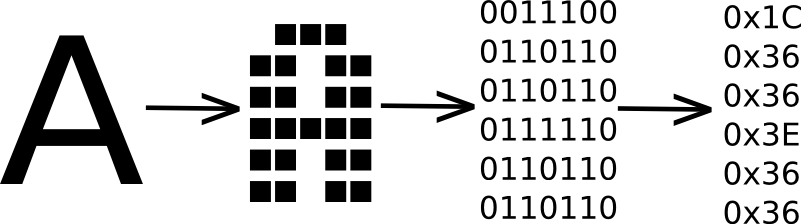
\includegraphics[width=15cm]{diagramafuente.png}}

Este fue el procedimiento para generar la fuente de 16x16 de la consola, el cual nos evita tener que realizar a mano cada carácter.
\begin{enumerate}
\item Se descargó de internet la fuente deseada, inspirada en la que usaban los juegos de la consola (formato ttf)
\item Se creó una imagen conteniendo todos los carácteres en una cuadricula (formato xfc)
\item Se exportó la imagen a formado RAW (extensión .data)
\item Se hizo makearray.cpp\footnote{en utils/fuentes}, que carga la imagen y para cada fila calcula una máscara de bits de sus pixeles y las muestra como un arreglo de C.
\item Se agregó el mismo al codigo fuente del kernel\footnote{graphics/rsrc/nesfont.h, usando en graphics/video.c}.	
\end{enumerate}

\section{Teclado}\label{sec:teclado}
Para detectar cuando se presiona una tecla, se configuró la interrupción IRQ1 para que llame a la función kbd\_handler\footnote{kernel/arch/x86/generic/drivers/keyboard.c}. En la misma se lee del puerto 0x60 para obtener el scancode que contiene información sobre si se soltó o presionó una tecla y cual fue.
La función getchar que proporciona el kernel se implementó usando una arreglo circular como buffer. Sin embargo esta función no es utilizada por el emulador ya que sólo necesita saber el estado de los controles en un momento dado.

\section{Administración de Memoria}\label{sec:memory}
En primer lugar, se dividió la memoria disponible en páginas de 4KB cada una. Se decidió utilizar la librería liballoc, cuyo funcionamiento se explica más adelante. La librería requiere que implementemos dos funciones: liballoc\_alloc y liballoc\_free\footnote{implementadas en kernel/arch/x86/pmm.c}.

\emph{liballoc\_alloc} recibe la cantidad de páginas contiguas que se necesitan reservar y debe devolver un puntero a la primer página.

\emph{liballoc\_free} es para liberar las páginas que reservamos anteriormente, recibe el puntero que habíamos devuelto y de alguna forma deberíamos marcar esas páginas como libres para ser reutilizadas.

Por cada página se guarda un bit, para saber si esa página está reservada (1) o libre (0). Como en cada entero podemos guardar 32 bits, podemos empaquetar todos los bits en $\lceil\frac{x}{32}\rceil=\lfloor\frac{x+31}{32}\rfloor$ enteros, donde x es la cantidad de páginas. Utilizando máscaras de bits podemos realizar las operaciones necesarias más rápidamente. En particular se necesitaron tres funciones auxiliares\footnote{implementadas en kernel/arch/x86/pmm.c}.

\begin{itemize}
\item bitmap\_set(l, r): Dado un intervalo en el bitset, setear todos los bits que estan dentro de él. Es usada para marcar las páginas como ocupadas.
\item bitmap\_clear(l, r): Análogo a la anterior, pero para limpiar los bits.
\item fits\_inside(x, v): Busca dentro de un entero v (32 bits) si hay x bits libres contiguos. 
\end{itemize}
Por ejemplo, para implementar bitmap\_set, primero se activaron los bits de los extremos usando máscaras de bits y luego los restantes mediante una lamada a memset. Se muestra un ejemplo en la figura ~\ref{fig:bitmap} (usando 8 bits en lugar de 32).

\begin{figure}[H]\caption{\label{fig:bitmap}}
\centering\def\svgwidth{\columnwidth}
\includesvg{bitmap_diagram}
\end{figure}
\subsection{liballoc}
Internamente para cada conjunto de páginas reservadas se crea un 'super bloque'. Cuando se llama a malloc se busca un super bloque con la suficiente memoria libre y se crea un bloque dentro de él, que va a contener la memoria que se va a otorgar al llamante.

Un dato interesante es que como estamos implementando malloc no podríamos pedir más memoria dinámica para guardar información sobre los bloques. La solución a esto fue guardar esta información directamente al comienzo de cada bloque. 
Para recorrer estas estructuras se usan listas enlazadas, los punteros al siguiente/anterior tambień se encuentran en las cabeceras de cada bloque, como se puede apreciar en la figura ~\ref{fig:liballoc}.

\begin{figure}[H]\caption{\label{fig:liballoc}}
\centering\def\svgwidth{\columnwidth}
\small\includesvg{liballoc_diagram}
\end{figure}

Otra ventaja de este sistema es que uando se recibe un puntero a la User Data, se puede acceder a su cabecera y obtener la información del bloque al que pertenece.

\section{Sistema virtual de archivos}\label{sec:vfs}
Necesitamos poder cargar los juegos desde algún lugar para poder emularlos. Como leer de discos puede ser relativamente complejo, se opto por un initrd\footnote{\url{http://en.wikipedia.org/wiki/Initrd}}. Esto es básicamente un archivo que se carga directamente en la RAM al inicio del sistema. Afortunadamente la carga de este archivo es realizada enteramente por GRUB antes de bootear el kernel. GRUB proporciona un puntero al inicio del archivo en RAM y el kernel se encarga de procesarlo.
\begin{figure}[H]\caption{\label{fig:initrd}}
\centering\def\svgwidth{\columnwidth}
\small\includesvg{initrd_diagram}
\end{figure}
 El formato del initrd que se utilizó se ejemplifica en la figura ~\ref{fig:initrd}. El mismo consta simplemente de los archivos colocados uno tras otro,junto con una cabecera que contiene el tamaño, nombre y un valor para verificar integridad.
 Para crear este initrd se programó initrd\_gen\footnote{utils/initrd\_gen.c}, el cual recibe los archivos y crea el la imagen lista para ser cargada por GRUB. En el archivo initrd.c\footnote{kernel/fs/initrd.c} se implementó la inicialización del initrd, junto con sus procedimientos para leer y listar los archivos.
 

